
\chapter{Introduction to Statistical Information Theory}
\section{What is Information?}


The first transistor was invented in 1947 at Bell Laboratories (Bell Labs), a research lab owned by AT\&T. It was the result of a collaboration between three scientists: John Bardeen, Walter Brattain, and William Shockley. The transistor, a small device capable of amplifying and switching electronic signals, replaced the bulky and less efficient vacuum tubes that were commonly used in radios and televisions. \bigskip


\begin{marginfigure}
    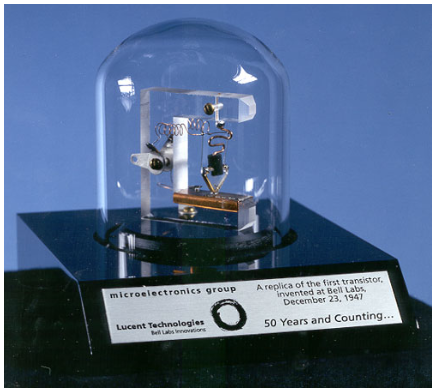
\includegraphics[width=\linewidth]{img/transistor.png}
    \caption{A replica of the first transistor, invented at Bell Labs in 1947.}
\end{marginfigure}


\begin{marginfigure}
    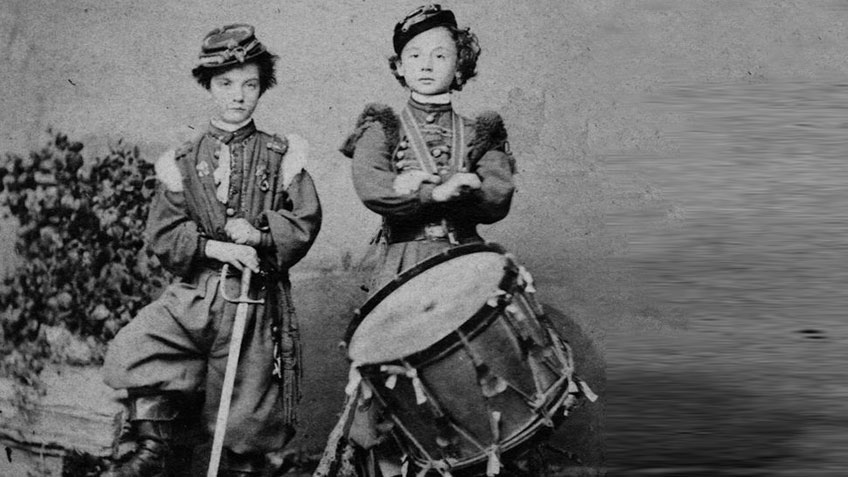
\includegraphics[width=\linewidth]{img/drummer.jpg}
    \caption{Drummer boys during the Civil War. Before radios and modern communication devices, verbal commands were difficult to hear on noisy battlefields. Drummer boys used rhythmic beats to communicate orders such as advance, retreat, or charge.}
\end{marginfigure}

\begin{marginfigure}
    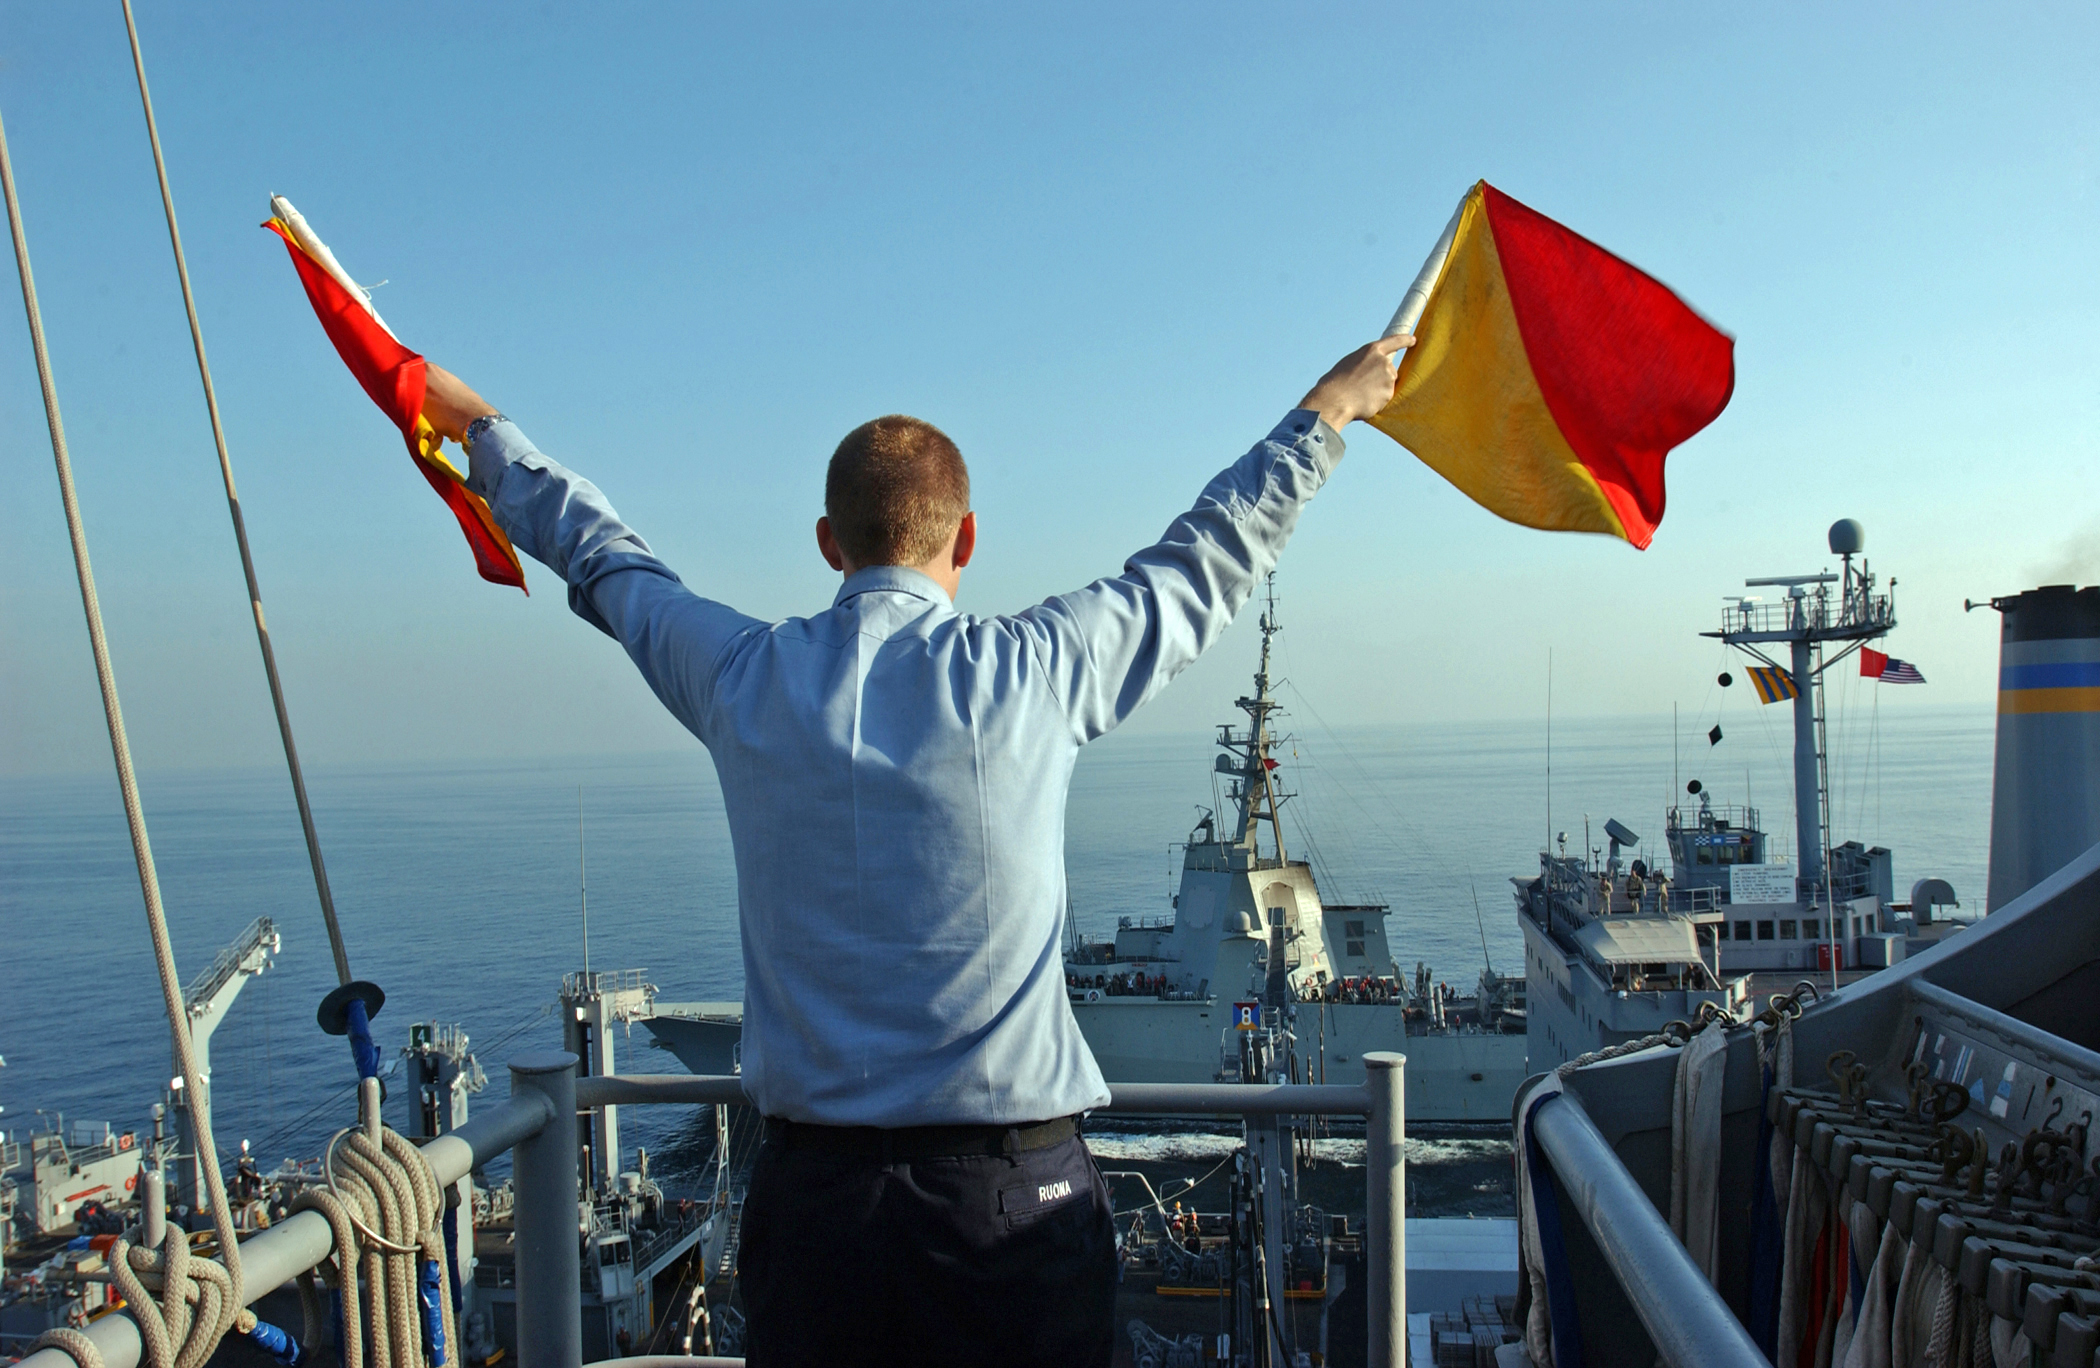
\includegraphics[width=\linewidth]{img/semaphores.jpg}
    \caption{Semaphore signalling is a method of visual communication using flags or lights. The system was invented in the 1790s by Claude Chappe, and was used for ships to communicate without radios. Semaphore flag signalling is still taught and used today in some maritime operations and by certain organisations like the Boy Scouts.}
\end{marginfigure}

Transistors could send messages to each other – but what exactly is the `information' being transmitted? \bigskip

In very early times, this information was identified with a physical object that carried it, e.g. a letter or carrier piegeon. It was later then carried by sound (military drums), and sometimes light (semaphores), and then electronic waves (radio).

\bigskip

It was Claude Shannon who turned the concept of information (which was a qualitative intuition) into a quantitative, mathematical construct that allows for optimisability.

\bigskip

\section{Enter Information Theory}

\defb{Fundamental Problem of Communication}{
    The fundamental problem of communication is that of reproducing at one point either exactly or approximately a message selected at another point. – Claude Shannon, 1948
    \begin{center}
        \resizebox{1\textwidth}{!}{
            \begin{tikzpicture}[node distance=2cm, thick]
                % Nodes (rectangles)
                \node[draw, rectangle, minimum width=2.5cm, minimum height=1cm] (source) {Information Source};
                \node[draw, rectangle, minimum width=2.5cm, minimum height=1cm, right=of source] (transmitter) {Transmitter};
                \node[draw, rectangle, minimum width=1cm, minimum height=1cm, right=of transmitter] (channel) {};
                \node[draw, rectangle, minimum width=2.5cm, minimum height=1cm, right=of channel] (receiver) {Receiver};
                \node[draw, rectangle, minimum width=2.5cm, minimum height=1cm, right=of receiver] (destination) {Destination};

                \node[draw, rectangle, minimum width=2.5cm, minimum height=1cm, below=of channel] (noise) {Noise Source};

                % Arrows
                \draw[->] (source) -- node[above]{Message} (transmitter);
                \draw[->] (transmitter) -- node[above]{Signal} (channel);
                \draw[->] (channel) -- node[align=center, above]{Received \\ Signal} (receiver);
                \draw[->] (receiver) -- node[above]{Message} (destination);

                \draw[->] (noise) -- (channel);
            \end{tikzpicture}
        }
    \end{center}
}


Upon successful completion of this module you will be able to:

\begin{itemize}
    \item Explain the key properties of information metrics in terms of communication principles.
    \item Calculate these metrics in common probability distributions.
    \item Compare different metrics and coding schemes on real-world data.
    \item Analyse the mathematical connections between data transmission and model fitting.
    \item Design principled data analysis plans with appropriate statistical criteria.
\end{itemize}

\subsection*{Part I: Source Coding (Compression)}
\begin{itemize}
    \item Information and probability
    \item Entropy and compression
    \item Source coding theorem
\end{itemize}

\subsection*{Part II: Channel Coding (Transmission)}
\begin{itemize}
    \item Mutual information and multivariate probability
    \item Channel codes
    \item Channel coding theorem
\end{itemize}

\subsection*{Part III: Statistics and Advanced Topics}
\begin{itemize}
    \item Model comparison and inference
    \item Estimating information from data
    \item Information decomposition
\end{itemize}


\refb{Main Textbook}{
    \textit{Information Theory, Inference, and Learning Algorithms}, by David MacKay.\\
    \url{http://www.inference.phy.cam.ac.uk/mackay/itila}
}

\refb{Additional Books}{
    \textit{Elements of Information Theory}, by T. Cover \& J. Thomas.\\
    \textit{Mathematics for Machine Learning}, by M. Deisenroth et al.\\
    \textit{Information Theory: A Tutorial Introduction}, by J. Stone.
}

\section{Sending a Message Reliably}
\begin{itemize}
    \item Alice goes to Japan and wants to send Bob a picture.
    \item Her connection is bad so it corrupts the image.
\end{itemize}
\begin{figure}[h]
    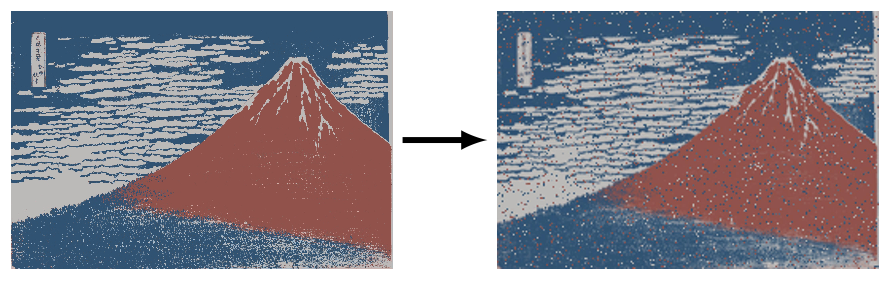
\includegraphics[width=\linewidth]{img/corrupt.png}
\end{figure}

\begin{itemize}
    \item\textbf{A physical solution:}
    \begin{itemize}
        \item Using a more reliable device.
        \item Moving to a zone with better signal.
        \item Communicating via cable.
    \end{itemize}
    \item\textbf{A system solution:}
    \begin{itemize}
        \item Build a system that can \textbf{detect} and \textbf{correct} errors. This is what we want.
    \end{itemize}
\end{itemize}

% System Solution Diagram
\resizebox{1\textwidth}{!}{
    \begin{tikzpicture}[node distance=2cm, thick]
        % Nodes (rectangles)
        \node[draw, rectangle, minimum width=2.5cm, minimum height=1cm] (source) {Information Source};
        \node[draw, rectangle, minimum width=2.5cm, minimum height=1cm, right=of source] (transmitter) {Transmitter};
        \node[draw, rectangle, minimum width=1cm, minimum height=1cm, right=of transmitter] (channel) {};
        \node[draw, rectangle, minimum width=2.5cm, minimum height=1cm, right=of channel] (receiver) {Receiver};
        \node[draw, rectangle, minimum width=2.5cm, minimum height=1cm, right=of receiver] (destination) {Destination};

        \node[draw, rectangle, minimum width=2.5cm, minimum height=1cm, below=of channel] (noise) {Noise Source};

        % Arrows
        \draw[->] (source) -- node[above]{Message} (transmitter);
        \draw[->] (transmitter) -- node[above]{Signal} (channel);
        \draw[->] (channel) -- node[align=center, above]{Received \\ Signal} (receiver);
        \draw[->] (receiver) -- node[above]{Message} (destination);

        \draw[->] (noise) -- (channel);
    \end{tikzpicture}

}

\section{A System Solution Example}
\subsection{Source Coding}

\begin{figure}[h]
    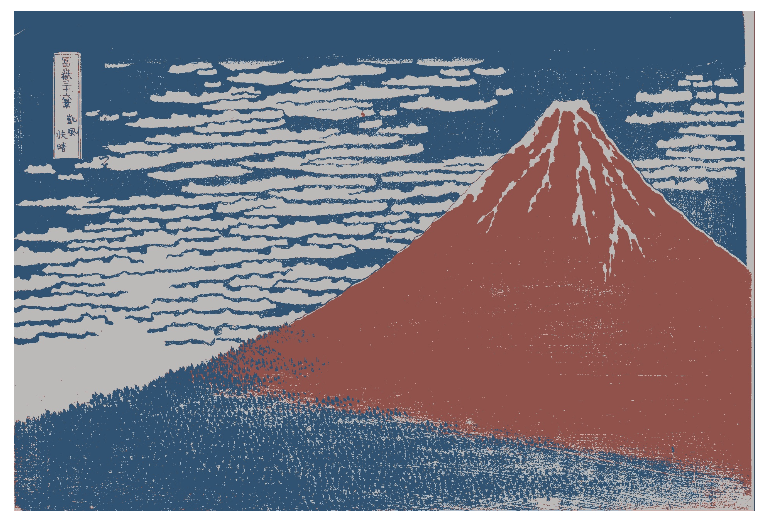
\includegraphics[width=\linewidth]{img/japan.png}
\end{figure}



We can build a map (code) of symbols to the data (\textcolor{red}{red}, \textcolor{blue}{blue}, \colorbox{black}{\textcolor{white}{white}}). Since we are working with electronics, the symbols we are allowed to transmit are (0,1), a binary.


\defb{A good code should be:}{
    \begin{enumerate}
        \item Short (i.e. few bits per pixel).
        \item Easily decodable (i.e. easy to invert).
    \end{enumerate}
}

\begin{enumerate}
    \item \textbf{Naive method: one-hot encoding.}
          \begin{itemize}
              \item On average, 3 bits per pixel.
          \end{itemize}
          \begin{center}
              \begin{tabular}{rcl}
                  \textcolor{blue}{Blue}                     & $\longrightarrow$ & 010 \\
                  \textcolor{red}{Red}                       & $\longrightarrow$ & 001 \\
                  \colorbox{black}{\textcolor{white}{White}} & $\longrightarrow$ & 100
              \end{tabular}
          \end{center}
    \item \textbf{Let's do better: Let more frequent symbols get shorter words (Huffman coding).}
          \begin{itemize}
              \item Assume that blue pixels occur most often, followed by red, and then white.
              \item On average, 1.56 bits per pixel.
          \end{itemize}
          \begin{center}
              \begin{tabular}{rcl}
                  \textcolor{blue}{Blue}                     & $\longrightarrow$ & 0  \\
                  \textcolor{red}{Red}                       & $\longrightarrow$ & 10 \\
                  \colorbox{black}{\textcolor{white}{White}} & $\longrightarrow$ & 11
              \end{tabular}
          \end{center}
\end{enumerate}

\subsection{Channel Coding}


\begin{itemize}
    \item Alice encodes the image into 0's and 1's and sends it over a channel.
    \item The channel has a probability \( f \) of flipping the message.
\end{itemize}



We can assign the probabilities with the following equations: \sidenote{
    This is known as the binary symmetric channel. Another view on probabilities:
    \begin{center}
        \begin{tabular}{c c c}
            \toprule
            $x$ & $y$ & $P(y \mid x)$ \\
            \midrule
            0   & 0   & $1 - f$       \\
            0   & 1   & $f$           \\
            1   & 0   & $f$           \\
            1   & 1   & $1 - f$       \\
            \bottomrule
        \end{tabular}
    \end{center}
}


\[
    \begin{tikzcd}[row sep=normal, column sep=normal]
        0 \arrow[r, ""] \arrow[dr, ""] & 0 \\
        1 \arrow[r, ""] \arrow[ur, ""] & 1
    \end{tikzcd}
    \quad
    \begin{aligned}
        P(y=0 \mid x=0) & = 1 - f; \quad & P(y=0 \mid x=1) & = f;    \\
        P(y=1 \mid x=0) & = f; \quad     & P(y=1 \mid x=1) & = 1 - f
    \end{aligned}
\]


\begin{itemize}
    \item One way we can reduce the error rate by flipping is the repeat the code, sending the same message multiple times.
\end{itemize}

\begin{center}
    \begin{tabular}{ll}
        \toprule
        \textbf{Source sequence ($s$)} & \textbf{Transmitted sequence ($t$)} \\
        \midrule
        0                              & 000                                 \\
        1                              & 111                                 \\
        \bottomrule
    \end{tabular}
\end{center}
\begin{itemize}
    \item The received sequence ($\mathbf{r}$) is transmission ($\mathbf{t}$) plus noise ($\mathbf{n}$):
\end{itemize}

\[
    \begin{array}{c|cccccccc}
        s & 0               & 0               & 1               & 0               & 1               & 1               & 0               \\
        t & \overbrace{000} & \overbrace{000} & \overbrace{111} & \overbrace{000} & \overbrace{111} & \overbrace{111} & \overbrace{000} \\
        n & 000             & 001             & 000             & 000             & 101             & 000             & 000             \\
        r & 000             & 001             & 111             & 000             & 010             & 111             & 000
    \end{array}
\]



\begin{itemize}
    \item When we receive the transmitted signal, we require a \textbf{decoder} to reconstruct the source signal.
    \item The optimal decoder is Bayes' rule:
          \[
              \hat{s} = \arg\max_s P(s \mid r_1 r_2 r_3) = \arg\max_s \frac{P(r_1 r_2 r_3 \mid s) P(s)}{P(r_1 r_2 r_3)}
          \]
    \item The optimal decoder is just the majority vote.
    \item Probability of making a \textbf{bit error} is:
          \[
              p_b = \text{probability of two flips} + \text{probability of three flips} = 3f^2 + f^3
          \]
    \item The error probability has decreased from $\mathcal{O}(f)$ to $\mathcal{O}(f^2)$ at the cost of reducing the communication rate by 3.

\end{itemize}

\begin{figure}[h]
    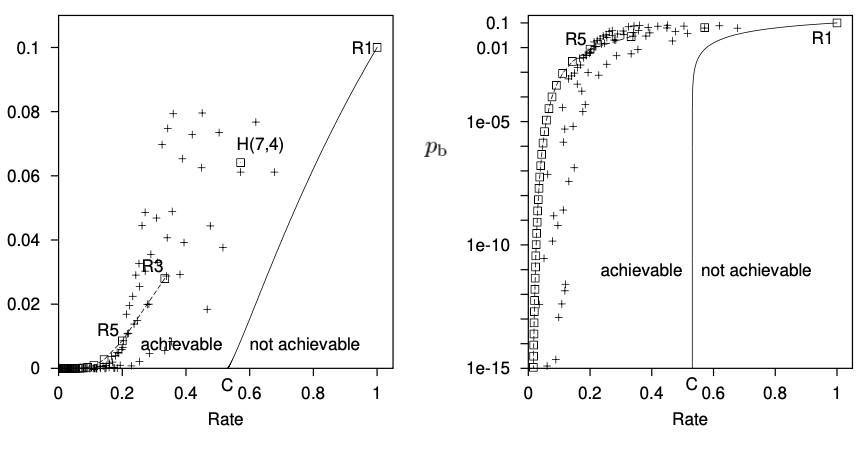
\includegraphics[width=\linewidth]{img/shannon-error-free.png}
    \caption{Achievable regions for error-free communication.}
    \label{fig:shannon-error-free}
\end{figure}

\begin{itemize}
    \item \textbf{Shannon's Channel Coding Theorem} shows that for rates \(R < C\) (channel capacity), error-free communication is possible with arbitrarily small bit error probability \(p_b\).
    \item As shown in Figure \ref{fig:shannon-error-free}, the \textit{achievable} region corresponds to rates where noise can be corrected with proper coding, while the \textit{non-achievable} region corresponds to rates \(R > C\), where reliable communication is impossible.
    \item \textbf{Key idea}: By using longer codewords and random coding, we can reduce \(p_b\) significantly, even in noisy channels, for rates less than \(C\).
    \item \textbf{Trade-off}: Lower rates allow more bits for error correction, enabling error-free transmission at the cost of reducing the communication rate.
\end{itemize}

\intuitb{Key takeaways}{
    Information theory is \textit{the art of redundancy}:
    \begin{itemize}
        \item removing redundancy when it hurts (compression),
        \item and adding redundancy when it helps (channel coding).
    \end{itemize}

    Information theory tells you what a statistical model \textit{can and cannot do}.
    \begin{itemize}
        \item Information and statistics are \textit{two sides of the same coin}.
    \end{itemize}
}


\section{Recap on Math}
\subsection{Sets and Functions}

\begin{itemize}
    \item A \textbf{set} is a mathematical word for ‘a collection of things’.
\end{itemize}

\subsubsection{Example Sets}
Weekdays: \( W := \{ \text{Mon, Tue, Wed, Thu, Fri, Sat, Sun} \} \). \\
Weekend: \( E := \{ \text{Sat, Sun} \} \).

\marginnote[40pt]{
    \textbf{All fun and games until...} \\
    \[ R = \{ S \mid S \not\in S \} \]
    This is the Russell’s Paradox, which posits that self-referencing sets create contradictions.
}

\begin{itemize}
    \item \textbf{Common set operations}:
          \begin{itemize}
              \item \textbf{Membership}: \( s \in S \iff s \) is an element of \( S \).
              \item \textbf{Subset}: \( R \subset S \iff \) all elements in \( R \) are in \( S \).
              \item \textbf{Complement}: \( S^c \) is the set of things not in \( S \).
              \item \textbf{Cardinality}: \( |S| \) is the number of elements in \( S \).
          \end{itemize}
\end{itemize}



\subsubsection{Functions}

\begin{itemize}
    \item A \textbf{function} \( f: X \to Y \) assigns an element of \( Y \) to each element of \( X \).
    \item A function is \textbf{injective} if \( f(x_1) = f(x_2) \implies x_1 = x_2 \).
    \item A function is \textbf{bijective} if it’s injective and \( \forall y \in Y \), \( \exists x \in X \) such that \( f(x) = y \).
\end{itemize}


\marginnote{
    \textbf{Bijective functions} are \textit{invertible}, meaning you can find a unique element in \( X \) for each element in \( Y \).
}
\begin{figure}[h]
    \begin{center}
        \begin{tikzpicture}[scale=0.8, >=Stealth]  % Sets arrowhead style to Stealth
            \node at (-3, 0.5) {Non-injective function};
            \node at (-3, -0.4) {X};
            \node at (0, -0.4) {Y};

            \draw (-3, -2) ellipse (1.2 and 2);
            \draw (0, -2) ellipse (1.2 and 2);

            \filldraw (-3,-3.4) circle (2pt);
            \filldraw (-3,-2.6) circle (2pt);
            \filldraw (-3,-1.8) circle (2pt);
            \filldraw (-3,-1.0) circle (2pt);

            \filldraw (0,-3.4) circle (2pt);
            \filldraw (0,-2.6) circle (2pt);
            \filldraw (0,-1.8) circle (2pt);
            \filldraw (0,-1.0) circle (2pt);

            \draw[->, >=Stealth, line width=0.8pt] (-3, -3.4) -- (0, -2.6);
            \draw[->, >=Stealth, line width=0.8pt] (-3, -2.6) -- (0, -2.6);
            \draw[->, >=Stealth, line width=0.8pt] (-3, -1.8) -- (0, -3.4);
            \draw[->, >=Stealth, line width=0.8pt] (-3, -1.0) -- (0, -1.8);

            \node at (4, 0.5) {Bijective function};
            \node at (4, -0.4) {X};
            \node at (7, -0.4) {Y};

            \draw (4, -2) ellipse (1.2 and 2.1);
            \draw (7, -2) ellipse (1.2 and 2.1);

            \filldraw (4,-3.4) circle (2pt);
            \filldraw (4,-2.6) circle (2pt);
            \filldraw (4,-1.8) circle (2pt);
            \filldraw (4,-1.0) circle (2pt);

            \filldraw (7,-3.4) circle (2pt);
            \filldraw (7,-2.6) circle (2pt);
            \filldraw (7,-1.8) circle (2pt);
            \filldraw (7,-1.0) circle (2pt);

            \draw[->, >=Stealth, line width=0.8pt] (4,-3.4) -- (7,-3.4);
            \draw[->, >=Stealth, line width=0.8pt] (4,-2.6) -- (7,-2.6);
            \draw[->, >=Stealth, line width=0.8pt] (4,-1.8) -- (7,-1.8);
            \draw[->, >=Stealth, line width=0.8pt] (4,-1.0) -- (7,-1.0);
        \end{tikzpicture}
    \end{center}
\end{figure}



\subsection{Logarithms}

\begin{itemize}
    \item The \textbf{logarithm} of a number \( x \), with base \( b \), is the power to which \( b \) must be raised to equal \( x \). That is:
          \[
              x = b^{\log_b(x)}
          \]
    \item In simpler terms, the logarithm is the inverse of the exponential function. For example, \( \log_2(8) = 3 \) because \( 2^3 = 8 \).
    \item Unless otherwise stated:
          \begin{itemize}
              \item \( \log \) means \( \log_2 \)
              \item \( \ln \) means \( \log_e \)
          \end{itemize}
\end{itemize}

Logarithms have many useful properties, such as:
\[
    \begin{aligned}
        \log_b(xy)  & = \log_b(x) + \log_b(y) \quad       & \text{(product rule)}           \\
        \log_b(x^n) & = n \log_b(x) \quad                 & \text{(power rule)}             \\
        \log_b(x)   & = \frac{\log_a(x)}{\log_a(b)} \quad & \text{(change of base formula)} \\
        \log_b(1)   & = 0 \quad                           & \text{(logarithm of 1)}
    \end{aligned}
\]



\sn{Potential Pitfall}{
    \( \log_b(x + y) \) is in general \textit{not} simplifiable.
}


\ex{log(8)}{
    \( \log(8) = 3 \), since \( 2^3 = 8 \).
}

\ex{log(1/8)}{
    \( \log(1/8) = -3 \), since \( \log(1/8) = \log(8^{-1}) = -\log(8) \).
}

\ex{ln(2)}{
    \( \ln(2) \approx 0.69 \) – you will be seeing this a lot!
}

\newpage
\subsection{Concavity and Convexity}

\begin{marginfigure}
    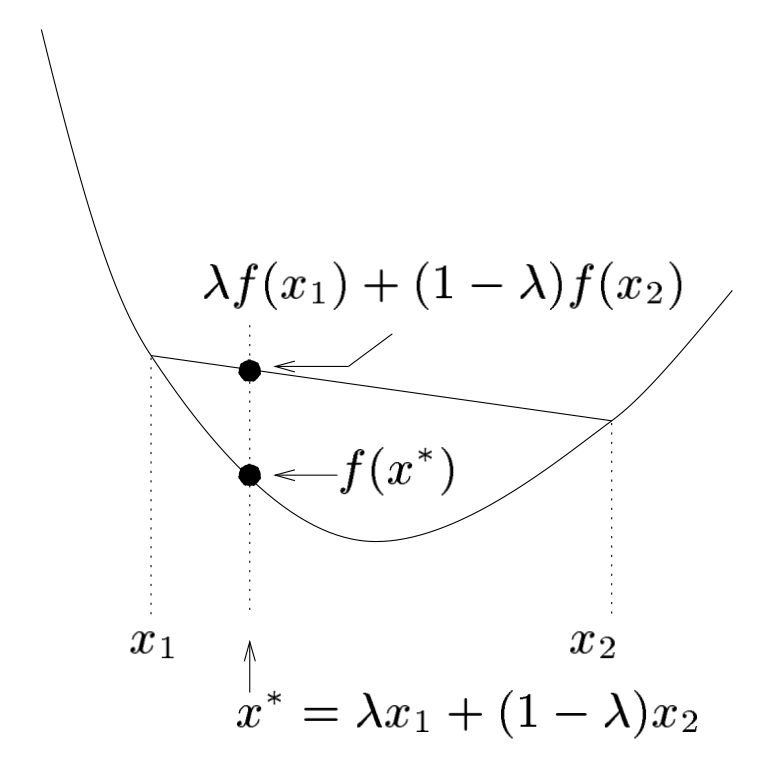
\includegraphics[width=\linewidth]{img/convex.png}
    \caption{A convex function.}
    \label{fig:convex}
\end{marginfigure}

A function is \textbf{convex} \textit{iff} a line between two points does not cross the function. Mathematically, this is represented as:
\[
    f(\lambda x_1 + (1-\lambda)x_2) \leq \lambda f(x_1) + (1-\lambda)f(x_2)
\]
for all \( x_1, x_2 \in \mathbb{R} \) and \( \lambda \in [0, 1] \). \bigskip

Similarly, a \textbf{concave} function is one where the inequality is reversed.

\marginnote[40pt]{Personally, the whole up-down mess is more a semantic issue, with elementary calculus textbooks using `concave up' and `concave down' to describe `convex' and `concave' functions respectively. For a longer thread: \href{https://math.stackexchange.com/questions/3399/why-does-convex-function-mean-concave-up}{Math StackExchange}.}
\sn{Concave or Convex?}{
    The terms convex and concave can be a bit confusing. We will specify:
    \[
        \text{Concave-up / Convex-down } (\cup) \text{ vs Concave-down / Convex-up } (\cap)
    \]

    In the grand scheme of things, convex refers to $\cup$ and concave refers to $\cap$.
}




\bigskip
To prove a function is convex, you can use the following approaches:

\begin{itemize}
    \item \textbf{Option 1:} Show the second derivative does not change sign.
    \item \textbf{Option 2:} Check if the function has \textit{convexity-preserving operations}:
          \begin{itemize}
              \item \textbf{Affine mapping:} If \( f(x) \) is convex, then \( f(Ax + b) \) is also convex.
              \item \textbf{Non-negative weighted sum:} If \( f_i(x) \) are convex and \( w_i \geq 0 \), then \( \sum_i w_i f_i(x) \) is convex.
              \item Many more.
          \end{itemize}
\end{itemize}

\refb{Convex Optimization by Boyd \& Vandenberghe}{
    \textit{Convex Optimization} is a highly recommended textbook for further reading.
}


\subsection{Concavity and Convexity}

\ex{Example: Concavity of the Logarithm}{
    The log and \( -x \log x \) are concave-down (\(\cap\)) functions.
    \begin{center}
        \begin{tikzpicture}
            \begin{axis}[
                    width=0.45\textwidth,
                    height=0.45\textwidth,
                    axis lines=middle,
                    xlabel={$x$},
                    ylabel={$ \log x $},
                    domain=0.01:4,
                    ymin=-2, ymax=2,
                    samples=100
                ]
                \addplot[thick, blue] {ln(x)};
            \end{axis}
            \begin{axis}[
                    width=0.45\textwidth,
                    height=0.45\textwidth,
                    axis lines=middle,
                    xlabel={$x$},
                    ylabel={$ -x \log x $},
                    domain=0.01:4,
                    ymin=-2, ymax=2,
                    xshift=6cm,
                    samples=100
                ]
                \addplot[thick, red] {-x*ln(x)};
            \end{axis}
        \end{tikzpicture}
    \end{center}
}

\subsection{Limits}

\defb{\ensuremath{(\epsilon, \delta)} Limit for 1D Functions}{

    A function \(f(x)\) tends to \(L\) as \(x\) tends to \(p\), written as:
    \[
        \lim_{x \to p} f(x) = L
    \]
    This means that for every \(\epsilon > 0\), there exists a \(\delta > 0\) such that for all \(x\), if \(0 < |x - p| < \delta\), then \(|f(x) - L| < \epsilon\).

    The \((\epsilon, \delta)\)-definition provides a rigorous way of understanding limits by ensuring that \(f(x)\) gets arbitrarily close to \(L\) when \(x\) is sufficiently close to \(p\), within the range controlled by \(\delta\).

}

\begin{marginfigure}[-150pt]
    \centering
    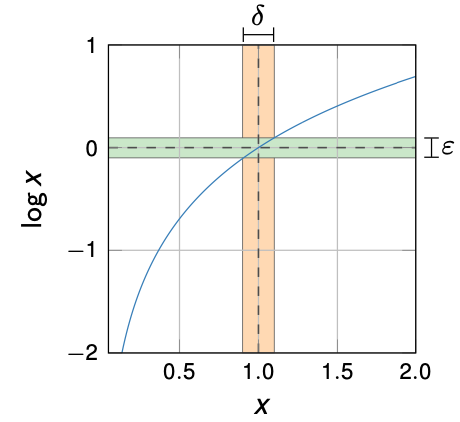
\includegraphics[width=1\textwidth]{img/eps_delta_limit_graph.png}
    \caption{Visual representation of the \((\epsilon, \delta)\)-definition for limits using \(\log x\).}
    \label{fig:eps_delta_log}
\end{marginfigure}

\ex{Example: \(\lim_{x \to 1} \ln(x) = 0\)}{
    To make \(\ln(x)\) within \(\epsilon\) of 0, \(x\) must be within \(\delta\) of 1.
    \begin{itemize}
        \item The closer \(x\) is to 1, the closer \(\ln(x)\) is to 0.
        \item We choose \(\delta\) to control how close \(x\) must be to 1.
    \end{itemize}
}

\defb{Infinite Limit Definition}{
    A function \(f(x)\) tends to \(\infty\) as \(x\) approaches \(p\), written as:
    \[
        \lim_{x \to p} f(x) = \infty
    \]
    This holds if, for every \(N > 0\), there exists a \(\delta > 0\) such that whenever \(0 < |x - p| < \delta\), we have \(f(x) > N\). The closer \(x\) is to \(p\), the larger \(f(x)\) becomes, growing beyond any pre-specified threshold \(N\).
}

\begin{marginfigure}[-150pt]
    \centering
    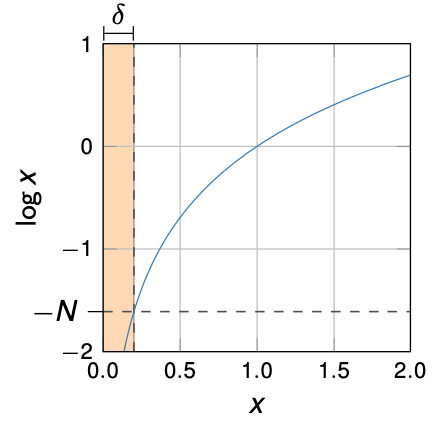
\includegraphics[width=1\textwidth]{img/infinite_limit_graph.png}
    \caption{Visualisation of the infinite limit behaviour using \(\log x\) as \(x\) approaches 0.}
    \label{fig:infinite_log_limit}
\end{marginfigure}

\ex{Example: \(\lim_{x \to 0^+} \ln(x) = -\infty\)}{
    To make \(\ln(x)\) smaller than \(-N\), \(x\) must be within \(\delta\) of 0 from the right.
    \begin{itemize}
        \item As \(x\) approaches 0 from the positive side, \(\ln(x)\) decreases without bound.
    \end{itemize}
}



\defb{Limit at Infinity}{

    A function \(f(x)\) tends to \(L\) as \(x\) tends to \(\infty\), written as:
    \[
        \lim_{x \to \infty} f(x) = L
    \]
    This means that for every \(\epsilon > 0\), there exists a constant \(c > 0\) such that whenever \(x > c\), we have \(|f(x) - L| < \epsilon\). In other words, as \(x\) becomes arbitrarily large, \(f(x)\) gets closer and closer to \(L\).
}
\begin{marginfigure}
    \centering
    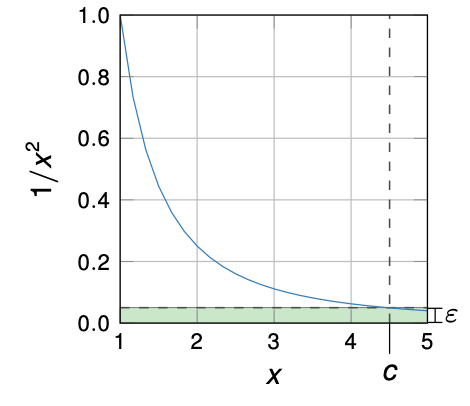
\includegraphics[width=1\textwidth]{img/limit_at_infinity_graph.png}
    \caption{Graph showing the limit at infinity using \(1/x^2\).}
    \label{fig:limit_infinity_1overx2}
\end{marginfigure}

\ex{Example: \(\lim_{x \to \infty} \frac{1}{x^2} = 0\)}{
    To make \(\frac{1}{x^2}\) within \(\epsilon\) of 0, \(x\) must be larger than some constant \(c\).
    \begin{itemize}
        \item The larger \(x\) is, the closer \(\frac{1}{x^2}\) gets to 0.
    \end{itemize}
}

\subsection{Random Variables}

A \textbf{random variable} is a mathematical concept used to represent any outcome that can take multiple values due to inherent randomness. Simply put, it is a "thing" that can take different values for reasons we may not fully know or control.

\defb{Random Variable Definition}{
    A random variable \(X\) is a measurable function \(X : \Omega \to E\), where:
    \begin{itemize}
        \item \(\Omega\) is the \textbf{sample space}, representing all possible outcomes of an experiment.
        \item \(E\) is the \textbf{event space}, representing all possible measurements associated with the outcomes.
        \item The random variable assigns a measurable outcome from \(\Omega\) to a corresponding value in \(E\).
    \end{itemize}
    This formal definition ensures that random variables are mathematically well-defined and that probabilities can be consistently assigned to the different values the variable might take.
}

\ex{Examples of Random Variables}{
    \begin{itemize}
        \item A \textbf{coin flip}, which can land heads or tails. Here, the random variable could represent the outcome (heads or tails).
        \item The \textbf{result of an election} before votes are cast. The random variable might represent the number of votes for each candidate.
        \item The \textbf{questions on an exam}. The random variable could model which questions are chosen randomly from a pool of possibilities.
    \end{itemize}
}

\defb{Ingredients of a Random Variable}{
    To define a random variable, we need three key components:
    \begin{itemize}
        \item The \textbf{sample space} (\(\Omega\)): the set of all possible outcomes of an experiment.
        \item The \textbf{event space} (\(E\)): the set of all possible measurements or values associated with each outcome.
        \item The \textbf{probability function} (\(P\)): assigns a probability to each outcome in the sample space. This ensures that the likelihood of different outcomes can be quantified.
    \end{itemize}
}

\ex{Example: Sequence of Coin Flips}{
    Consider an experiment where we toss three coins and count the number of heads:
    \begin{itemize}
        \item The sample space is \(\Omega = \{ H, T \}^3\), representing all possible combinations of heads and tails.
        \item The event space is \(E = \{ 0, 1, 2, 3 \}\), where each value corresponds to the number of heads observed.
        \item The random variable \(X\) is the \textbf{heads-counting function}, mapping outcomes to the number of heads:
        \[
            X(ttt) = 0, \quad X(tht) = 1, \quad X(thh) = 2, \quad X(hht) = 2, \dots
        \]
    \end{itemize}
}


One important requirement of any probability function associated with random variables is that the probabilities must be non-negative and must sum to 1. 
\[
    \forall \omega \in \Omega, \quad P(\omega) \geq 0 \quad \text{and} \quad P(\Omega) = 1
\]
This ensures that every possible outcome has a valid probability assigned to it, and that the total probability over all possible outcomes is 1, representing certainty that some outcome in \(\Omega\) will occur.


\subsection{Types of Random Variables}

Random variables can be classified based on the nature of the event space \(E\):

\begin{itemize}
    \item \textbf{Discrete:} If \(E\) is countable and finite, we call the random variable \textit{discrete}. This means that the set of possible values that the random variable can take is finite or countable.
    \item \textbf{Continuous:} If \(E \subseteq \mathbb{R}^d\), the random variable is \textit{continuous}. This means that the possible values lie in a continuous range, such as all real numbers between certain bounds.
\end{itemize}

We often refer to the event space \(E\) as the \textbf{alphabet} of the random variable \(X\), and denote it as \(\mathcal{X}\). This alphabet represents the set of all possible values that the random variable can take.

\vspace{1em}

\textbf{Notation Overview:}

To simplify our discussions about random variables, we will use the following notation:

\begin{table}[h]
    \centering
    \begin{tabular}{ll}
        \toprule
        \textbf{Symbol} & \textbf{Meaning} \\
        \midrule
        \(X\) (upper case) & Random variable \\
        \(x\) (lower case) & Particular value (or realisation) of \(X\) \\
        \(\mathcal{X}\) (squiggly) & Alphabet (possible values of \(x\)) \\
        \(X \sim p(x)\) & \(X\) is distributed according to \(p\) \\
        \(p(X = x_i), p(x_i), p_i\) & Probability of event \(x_i\) \\
        \bottomrule
    \end{tabular}
    \caption{Notation for Random Variables}
\end{table}

\vspace{1em}

\intuitb{Key Points to Remember:}{
\begin{itemize}
    \item \(\mathcal{X}\) is the set of all possible outcomes (values) of a random variable \(X\). It can either be discrete or continuous.
    \item \(X\) represents the random variable as a whole, while \(x\) represents a specific realisation or value that \(X\) can take.
    \item The distribution \(p(x)\) tells us how likely it is for \(X\) to take each value in \(\mathcal{X}\).
\end{itemize}
}

\subsection{Probability Distributions}

Random variables can be described by their \textbf{probability distributions}. The type of probability distribution depends on the nature of the random variable \(X\):

\begin{itemize}
    \item \textbf{Discrete:} For a discrete random variable, we use the \textbf{probability mass function} (PMF). The total probability for all possible values of \(X\) must sum to 1:
    \[
    \sum_{x \in \mathcal{X}} P(X = x) = 1
    \]
    \item \textbf{Continuous:} For a continuous random variable, we use the \textbf{probability density function} (PDF). The integral of the PDF over the entire range of possible values must equal 1:
    \[
    \int_{\mathcal{X}} p(x) \, dx = 1
    \]
\end{itemize}

Both of these are often referred to as the \textbf{probability distribution function} (PDF) in a general sense, though it should be clear from the context whether we mean a probability mass function (discrete) or a probability density function (continuous).

\vspace{1em}

\sn{Probability Higher than 1?}{
For \textbf{density} functions, it is possible for the function value to be greater than 1 at certain points. However, the integral over any interval \(a \leq x \leq b\) must still be less than or equal to 1:
\[
\int_a^b p(x) \, dx \leq 1
\]
This ensures that the total probability remains valid, even if the function exceeds 1 at specific values of \(x\).

}

\vspace{2em}

\subsection{Expected Value}

The \textbf{expected value} of a random variable \(X\) is the long-run average value that \(X\) takes when considering its probability distribution. For a given random variable \(X \sim p(x)\) and a function \(f\), the expected value of \(f(X)\) under the distribution \(p\) is:

\[
\mathbb{E}_p[f(X)] := \sum_{x \in \mathcal{X}} p(x) f(x)
\]

When the probability distribution is clear from context, we can omit \(p\) and simply write the expectation as \(\mathbb{E}[f(X)]\).

\begin{itemize}
    \item \textbf{Mean of \(X\):} The mean is the expected value of the random variable itself:
    \[
    \mathbb{E}[X]
    \]
    \item \textbf{Variance of \(X\):} The variance measures the spread of the random variable around its mean:
    \[
    \mathbb{E}[(X - \mu)^2] = \mathbb{E}[X^2] - \mu^2
    \]
\end{itemize}


\subsection{Probability Distributions}

\thm{Jensen's Inequality}{
    Let \( f \) be a convex function and let \( X \) be a random variable with a probability distribution \( p(x) \). Jensen's inequality states that:
    \[
        f(\mathbb{E}[X]) \leq \mathbb{E}[f(X)] 
    \]
}

\subsubsection{Proof of Jensen's Inequality (for the Discrete Case):} 

Let \( X \) be a discrete random variable taking values \( x_1, x_2, \dots, x_n \) with probabilities \( p_1, p_2, \dots, p_n \), where \( 0 \leq p_i \leq 1 \) and \( \sum_{i=1}^n p_i = 1 \).

We will prove the inequality by induction on \( n \), the number of possible values of \( X \).

\smallskip \textbf{Base Case (\( n = 1 \)):} \smallskip

When \( n = 1 \), \( X \) takes a single value \( x_1 \) with probability \( p_1 = 1 \). Then:
\[
    \mathbb{E}[f(X)] = f(x_1), \quad \mathbb{E}[X] = x_1, \quad \text{so} \quad \mathbb{E}[f(X)] = f(\mathbb{E}[X])
\]
Thus, the inequality holds with equality.

\smallskip \textbf{Inductive Step:} \smallskip

Assume that Jensen's inequality holds for any discrete random variable taking \( n-1 \) values.

Consider \( X \) taking \( n \) values \( x_1, x_2, \dots, x_n \) with probabilities \( p_1, p_2, \dots, p_n \).

The expected value of \( X \) is:
\[
    \mathbb{E}[X] = p_1x_1 + \sum_{i=2}^{n} p_i x_i \quad \text{where } p_1 \in [0, 1]
\]

Define \( P = \sum_{i=2}^{n} p_i = 1 - p_1 \) and \( \mu = \frac{1}{P} \sum_{i=2}^{n} p_i x_i \). Then:
\[
    \mathbb{E}[X] = p_1 x_1 + P \mu \quad \text{where } p_1, P \in [0, 1]
\]

By the convexity of \( f \) and knowing that \( p_1 + P = 1 \), we have:
\begin{align*}
    f(\mathbb{E}[X]) &= f(p_1 x_1 + P \mu) \\
    &\leq p_1 f(x_1) + P f(\mu) \quad \text{(by convexity of } f\text{)}
\end{align*}

By the induction hypothesis, applied to the \( n-1 \) values \( x_2, x_3, \dots, x_n \) with adjusted probabilities \( \frac{p_i}{P} \) for \( i = 2, \dots, n \), we have:
\[
    \sum_{i=2}^{n} \frac{p_i}{P} f(x_i) \leq f\left( \frac{1}{P} \sum_{i=2}^{n} p_i x_i \right) = f(\mu)
\]
Multiplying both sides by \( P \):
\[
    \sum_{i=2}^{n} p_i f(x_i) \leq P f(\mu)
\]

Adding \( p_1 f(x_1) \) to both sides:
\[
    \sum_{i=1}^{n} p_i f(x_i) \leq p_1 f(x_1) + P f(\mu)
\]
From the earlier inequality:
\[
    f(\mathbb{E}[X]) \leq p_1 f(x_1) + P f(\mu) \leq \sum_{i=1}^{n} p_i f(x_i) = \mathbb{E}[f(X)]
\]
Thus, the inequality holds for \( n \) values.





\subsection{The Normal Distribution}

\defb{Definition: Normal (or Gaussian) Distribution}{
The probability density function (PDF) for the \(d\)-dimensional normal distribution with mean \(\mu\) and covariance \(\Sigma\), denoted by \(\mathcal{N}(\mu, \Sigma)\), is:

\[
p(x; \mu, \Sigma) = (2\pi)^{-d/2} |\Sigma|^{-1/2} \exp \left( -\frac{1}{2} (x - \mu)^\top \Sigma^{-1} (x - \mu) \right)
\]
}
\begin{figure}[h]
    \centering
    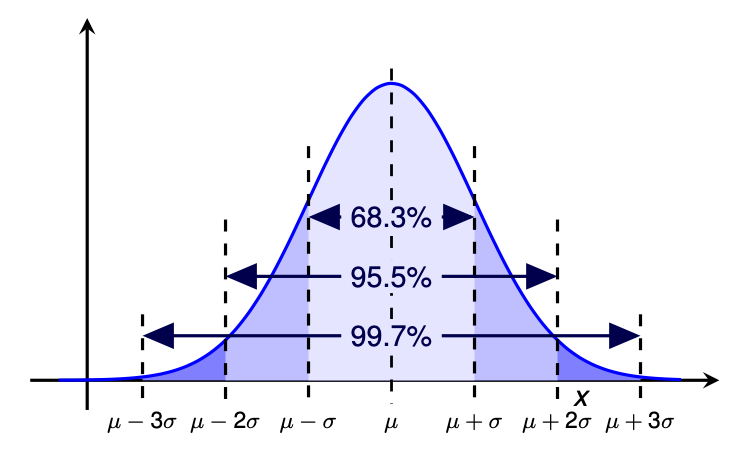
\includegraphics[width=0.6\linewidth]{img/normal_dist.png}
    \caption{The Normal Distribution curve, with highlights of the percentages of data within \(1\sigma\), \(2\sigma\), and \(3\sigma\) from the mean.}
\end{figure}


\section{Summary}

\begin{itemize}
    \item \textbf{Course aims:}
    \begin{itemize}
        \item Information theory as a unified language for statistics, communications, and geometry.
        \item Useful for studying the limitations and possibilities of statistical models.
    \end{itemize}

    \item \textbf{Relevant mathematical concepts:}
    \begin{itemize}
        \item Probability distributions and random variables.
        \item Convexity/concavity and Jensen's inequality.
    \end{itemize}
\end{itemize}
